\documentclass{article}
\usepackage[utf8]{inputenc}

\usepackage{amsmath}
\usepackage{amssymb}
\usepackage{graphicx}

\title{Variational Recurrent Neural Networks}
\author{Sukuru Sai Vineet}

\begin{document}

\maketitle

\section{Introduction}
Recurrent Neural Networks are the standard model to use for sequential data. However these RNNs usually use a deterministic function to update the hidden state:

\[ h_{t} =f (x_{t}, h_{t - 1}) \]

Where $ f $ is parametrized in a non linear fashion with some tensor $ \theta $

The deterministic nature of this equation leads to low variability in the outputs of the RNN. All variability is obtained from either the sampling step (sampling from the probability distribution produced by the RNN every timestep) or from variability in the input $ x_t $ itself.

To provide variability this paper provides an architecture that is based on the idea of Variational Autoencoders (VAEs).

\section{Variational Autoencoders}

Variational Autoencoders are a family of generative models. The main idea is to generate data that is part
of a probability distribution using an intermediate random variable called the latent variable. We do not explain the full architecture here, only the parts that are utilised in the recurrent model presented.

To learn a probabilility distribution $ P(X) $ we factorize it as follows

\begin{equation*}
    P(X) = P(X|z)P(z)
\end{equation*}

Where $ z $ is known as a latent variable. We consider $ z \sim \mathcal{N}(0,\,1)\, $ for sake of mathematical and curve fitting convenience.

To fit these potentially complicated probability distributions we use a neural network architecture that is end to end differentiable. See attached figure.

The objective function (to be maximised via backprop and gradient ascent algorithms) used for training is as follows

\begin{equation*}
    - KL ( Q (z | X) || P(z) ) + \mathbb{E}_{Q(z | X)}
                                            log( P ( X | z ) )
\end{equation*}

Where KL is the Kullback-Leibler diveregence between the 
reparametrized encoder network $ Q(z|X) $ and the prior 
gaussian $ P(z) $ and the other term being the probability of real distribution given latent distribution

The second log probability term is supposed to encourage the network to produce more real
looking distributions from the latent variable. It is maximizing the log likelihood of
the real distribution given the latent variable.
while the KL divergence term acts as regularization. If we use only log likelihood, the network
will produce a sort of "average" of all the data it has been given to maximise log probability, which is undesirable.
To prevent this $ Q(z|X) $ returns the probability that a given $ z $ latent variable will be able to generate a good distribution
for $ X $ and we train this so the information loss between the prior and the latent space is small, so simpler latent representations are encouraged.

With this bag of tricks, we move onto making VAEs recurrent in nature.

\begin{figure}[h!]
    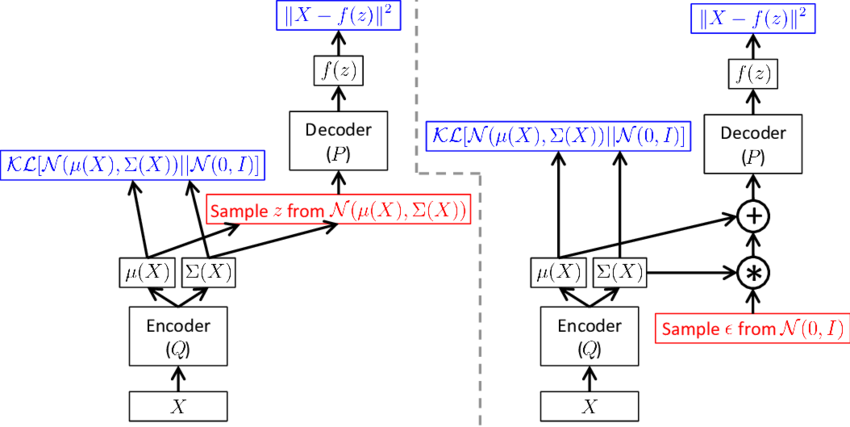
\includegraphics{VAENetwork.jpg}
    \caption{Network implementation with reparametrization trick}
    \label{fig:fig1}
\end{figure}

\section{Variational Recurrent Neural Network}

Essentially, every time step of an RNN being a VAE leads to the model of a Variational RNN.

The factorization that motivates this architecture is

\[ 
   P(x_{\le T}) = \prod_{t=1}^{t=T} P(x_t | z_{\le t},x{\le t}) 
                                    P (z_t | x_{<t}, z_{<t})
\]

To incorporate the information received in previous timesteps into $ z_t $ we condition it on a prior that is calculated from $ h_{t-1} $, thus
we can obtain a reparametrized trick version of the second term in the above product.

The first term is obtained through a regular VAE structure that encodes and decodes, going through the latent variable $ z_t $ 

There are multiple subnetworks at play in one timestep of a VRNN. They are as follows

\begin{enumerate}
    \item{ $ \phi_{prior}(h_{t-1}) $ : Generates the prior means and 
        standard deviations to condition $ z_t $ against. }
    \item{ $ \phi_{encoder}(x_t, h_{t-1}) $ : Generate $ z_t $ means 
        and standard deviations. Note that it nows takes 
        $ h_{t-1} $ so that we can 
        condition $ z_t $ on all $ x_{\le t} $ }
    \item{ $ \phi_{decoder}(z_t, h_{t-1}) $ : Generate log 
        probability $ log P( x_{t} | z_{\le t}, x_{<t} ) $
        }
    \item{
            $ \phi_{hidden}(x_t, z_t, h_{t-1}) $ : Generate $ h_t $.
            Note that due to recurrence, this hidden state has the capability
            to incorporate the information $ x_{\le t} $ and $ z_{\le t} $
            which makes prior conditioning work.
        }
\end{enumerate}

The objective function for each timestep looks very similar to a normal VAE
\[
    - KL(q(z_t | x_{\le t}, z_{<t}) || P(z_t | x_{<t}, z_{<t} ))
    + log P(x_t | z_{\le t}, x_{<t})
\]

This is averaged across all timesteps to approximate the expectation.

\section{Results}

VRNNs are good at modelling data that have short term variations but long term patterns, such as
speech and handwriting.

\end{document}
